\documentclass{article}
\usepackage{hyperref}
\usepackage{tabularx}
\usepackage{graphicx}
\usepackage{enumerate}
\usepackage{listings}
\usepackage{float}

\begin{document}

\title{11-792 Project Report}

\author{Nicholas Gekakis, Boyue Li}

\maketitle

\section{Overview}

In this project, we built a distributed parallel configuration space exploration pipeline framework,
which can exhaustively try all possible parameter combinations automatically.
Users can easily configure multiple modules,
create their own modules and run on multiple processes or even multiple machines.

\section{Requirements}

    \subsection{Easy to configure and deploy}
    The framework should be easy to configure and deploy.

    \subsection{Save and resume}
    The framework should be able to save intermediate results so that it can be interrupted and resume running at a later time.

    \subsection{Automatical parameter exploring}
    The framework should be able to automatically execute using all possible parameter combinations that have been configured by the pipeline developers.

    \subsection{Easy to develop users' modules}
    The framwork should support a easy way for users to develop their own modules.

    \subsection{Load balancing}
    The framework should be able to handle load balancing since different modules require different excution time.

\section{Design}

    \subsection{Overview}

    As shown in Fig. \ref{fig:control_flow},
    a pipeline is constructed from several independent modules.
    A module reads data from the data server,
    processes data according to all possible parameters,
    then save results for each configuration to the data server.

    \begin{figure}[h]
        \begin{center}
            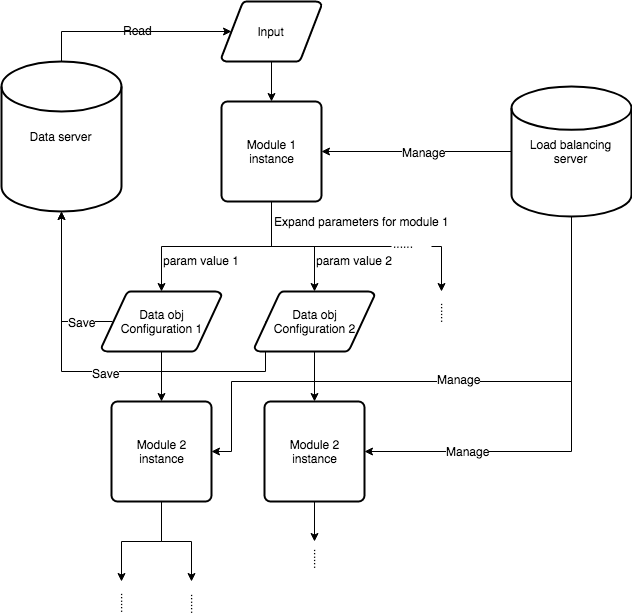
\includegraphics[width=\textwidth]{fig/control_flow.png}
        \end{center}
        \label{fig:control_flow}
        \caption{Control flowchart.}
    \end{figure}

    \begin{figure}[h]
        \begin{center}
            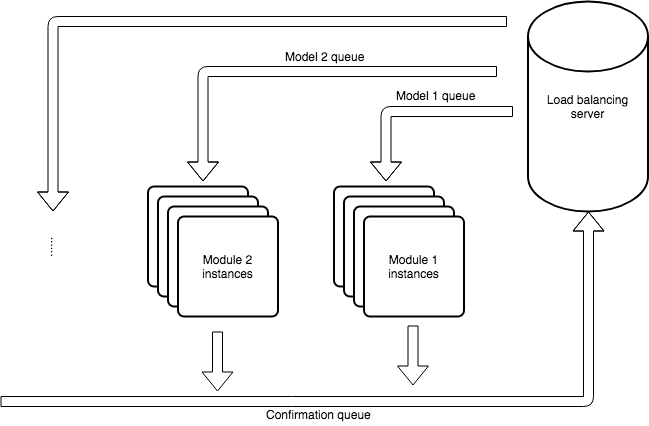
\includegraphics[width=\textwidth]{fig/information_flow.png}
        \end{center}
        \label{fig:information_flow}
        \caption{Information flowchart.}
    \end{figure}


    Every module runs on an independent process
    and communicates through RabbitMQ using the job class (defined in section \ref{sec:job}) which contains parameters, current excuetion status and the path to input file.
    Fig. \ref{fig:information_flow} describes the information flow.
    Load balancing server distributes jobs to different modules' instances.
    Once the job is finished, the instance send a confirmation to the load balancing server.


    Users only need to specify the connections between modules and the parameters every module needs,
    the framework will automatically handle execution and configuration space exploration.

    \begin{figure}[H]
        \begin{center}
            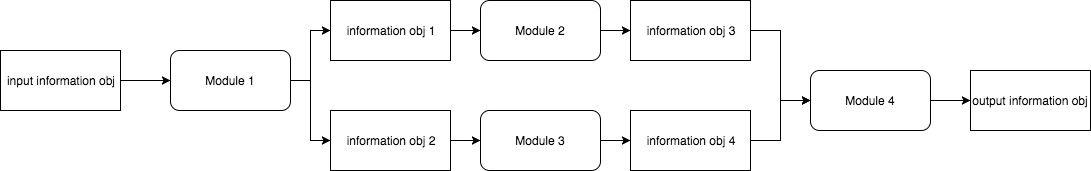
\includegraphics[width=1.2\textwidth]{fig/sample_pipeline.png}
        \end{center}
        \label{fig:sample_pipeline}
        \caption{A sample pipeline}
    \end{figure}
    Figure \ref{fig:sample_pipeline} shows a sample pipeline which passes the input information object
    through some modules and produces the output information object.

    We also provided a command line executable, to ease users' pain of coding.


    \subsection{Pipeline}
    The pipeline class manages modules and parameters.
    It reads configuration file, creates the pipeline and is the actual class for the load balancing server.
    The pipeline can't have branches or merges, and the order of the configuration file should be the same with the actual pipeline.

    \begin{figure}[h]
        \begin{center}
            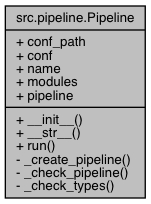
\includegraphics[width=0.3\textwidth]{fig/pipeline_uml.png}
        \end{center}
        \label{fig:pipeline_uml}
        \caption{UML diagram for the pipeline class.}
    \end{figure}

    \subsection{Module}
    A module is the basic computation unit which takes an input and produces an output.
    Every input and output is an job object defined in sec. \ref{sec:job}.

    A module needs to maintain the following fields:
    \begin{itemize}
        \item Name of the module.
        \item Number of instances.
        \item Configuration of the pipeline.
    \end{itemize}
        
    When running, the pipeline will send jobs to module instances.

    \begin{figure}[H]
        \begin{center}
            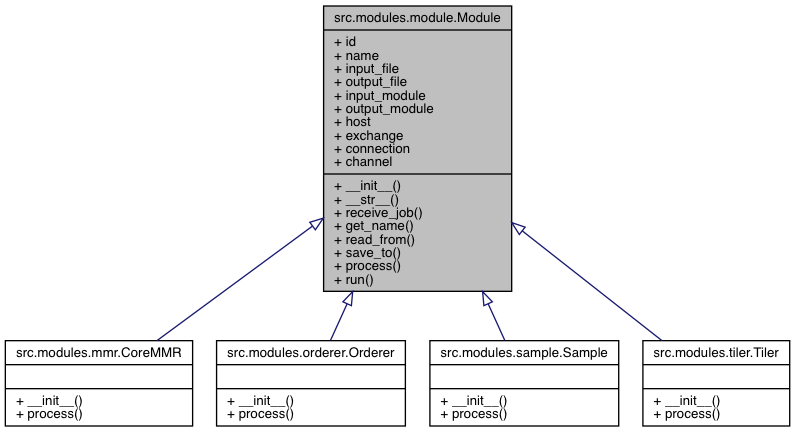
\includegraphics[width=0.4\textwidth]{fig/module_uml.png}
        \end{center}
        \label{fig:module_uml}
        \caption{UML diagrams for the abstract module class and derived classes.}
    \end{figure}

    \subsection{Parameter}
    \label{sec:parameter}
    The parameter class manages one parameter.
    It should handle all operations related the parameter,
    including updating the parameter value,
    set and reset the value.
    There are several types of params: integer, float and collection.

    It also needs to save maintain the following fileds:
    \begin{itemize}
        \item Name of the parameter.
        \item Type of the parameter: int, float or collection.
        \item Interval of possible values or possible values of a collection.
        \item Step size of the parameter (for numerical params).
    \end{itemize}

    \begin{figure}[H]
        \begin{center}
            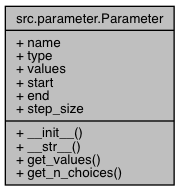
\includegraphics[width=0.3\textwidth]{fig/param_uml.png}
        \end{center}
        \label{fig:param_uml}
        \caption{UML diagram for parameter class.}
    \end{figure}

    \subsection{Job}
    \label{sec:job}
    The job class is the information object used between modules.
    It maintains the following fileds:

    \begin{itemize}
        \item Job id: the unique id of the job.
        \item Producer: the module that produced this information object.
        \item Consumer: the module that this information object to be passed to.
        \item Input uri: the uri to the data file.
        \item Output path: the path to store the resulting data file.
        \item Params: the params that the module should use to process the data object.
        \item Timestample: the timestamp when the data object was created.
        \item Processing time: the time taken to process the data object.
    \end{itemize}


    \begin{figure}[H]
        \begin{center}
            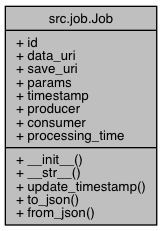
\includegraphics[width=0.3\textwidth]{fig/job_uml.png}
        \end{center}
        \label{fig:job_uml}
        \caption{UML diagram for job class.}
    \end{figure}


    \subsection{Configuration file}
    We use YAML files to configure the framework.

    \subsection{User defined modules}
    Users need to put their module classes in a file in the same folder with the configuration file.
    Then the framework will automatically load them.

    \subsection{Executable}
    We provide an executable that reads in the configuration file, and runs all possible configurations.


\section{Example pipeline}
    This pipeline consists of a sample module,
    which does nothing but adds its own configuration and parameters to the data to show this pipeline is working.

    \begin{figure}[H]
        \begin{center}
            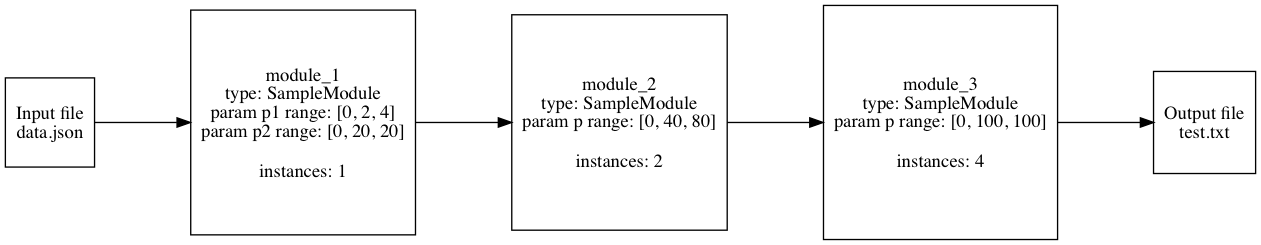
\includegraphics[width=1.2\textwidth]{fig/toy_pipeline.png}
        \end{center}
        \label{fig:toy_pipeline}
        \caption{The structure for toy pipeline}
    \end{figure}


\section{Experiments}

    \subsection{Dataset}
    The results were run on a subset (100 total questions) of the bioasq\_train\_formatted.json dataset.

    \subsection{Pipeline}

    \begin{figure}[H]
        \begin{center}
            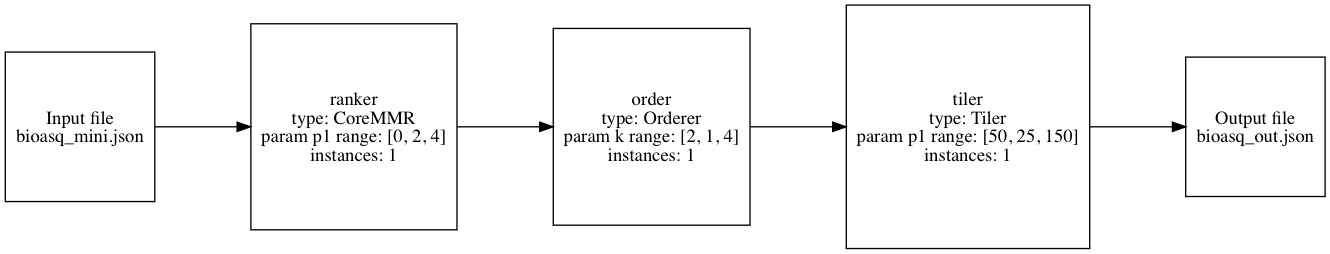
\includegraphics[width=\textwidth]{fig/bioasq_pipeline.png}
        \end{center}
        \label{fig:bioasq_pipeline}
        \caption{The structure for BioAsq pipeline}
    \end{figure}


    \section{Implemented Modules}

        Table \ref{tbl:modules} listed all modules and their parameters we implemented.
        We have also improvemented the existing BioASQ code a lot.
        We made a multi-process CoreMMR module, that is more than 4x faster than the original module (also depending the configuration).

        \begin{table}[h]
            \centering
            \begin{tabular}{|l|l|}
                \hline
                Module  & Parameters \\ \hline
                CoreMMR & $\alpha$           \\ \hline
                Orderer &  k          \\ \hline
                Tiler   &  word\_limit          \\ \hline
                Rouge   &            \\ \hline
            \end{tabular}
            \caption{Table of implemented modules.}
            \label{tbl:modules}
        \end{table}

    \subsection{Results}
    %Our experimental results show that the best configuration uses the following parameters: alpha=0.65, k=2, word limit=100.


\section*{Acknowledgements}
Thanks for Khyathi's help.

\end{document}
